\section{\LaTeX~Coding Best Practices} \label{sec:Conclusion}
This section outlines some key packages and functions that are extremely helpful when working with \href{https://www.latex-project.org/}{\LaTeX}. 
For readers new to \LaTeX\, ``LaTeX\ is a high-quality typesetting system; it includes features designed for the production of technical and scientific documentation,'' \cite{latexExplanation}. 
\LaTeX\ is written via the use of an editing software. 
Common editing programs include \href{https://www.overleaf.com/}{OverLeaf} for online usage, or \href{https://miktex.org/}{Mik\TeX} with \href{https://www.texstudio.org/}{\TeX studio} for offline usage. 

\subsection{Document Setup}
Long \LaTeX\ documents become very confusing, very quickly if a proper file structure is not established. 
\LaTeX\ uses one document to import required packages, set formats, and generate a .PDF document. 
It is suggested to use the main \LaTeX\ document only for the global packages, and the calling of subsequent document files. 
Therefore, limited writing should occur within the main \LaTeX\ file. 
Sections of a document should be individual files, added to the main file via the command \verb*|\input{}|. 
An example file structure, with \LaTeX\ files in the main folder, and supporting photos and resources in sub-folders, is presented in \cref{fig:documentSetupExample}.


\begin{figure}[hbt!]
	\centering
	\captionsetup{width=0.6\textwidth}
	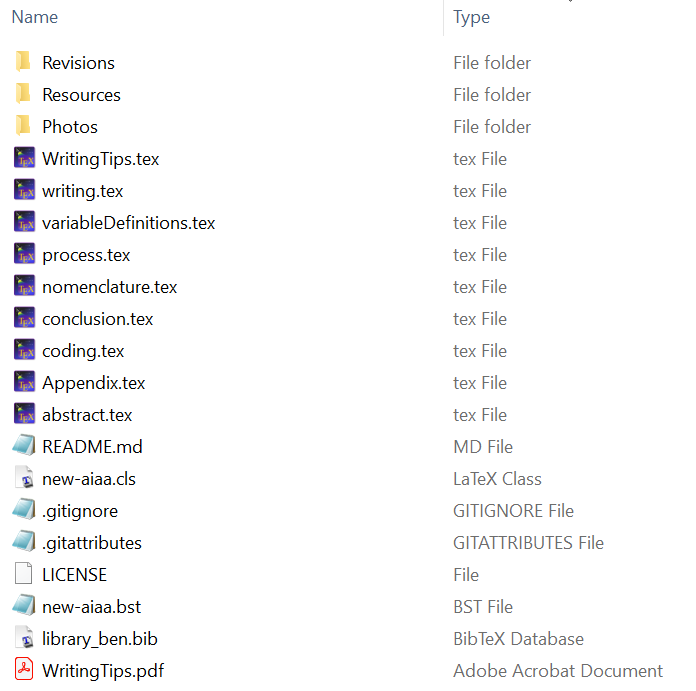
\includegraphics[width=0.6\textwidth]{Photos/Figures/projectStructure.png}
	\caption{Example file structure for a \LaTeX\ document project.}
	\label{fig:documentSetupExample}
	\hfill
\end{figure}

\noindent
In \cref{fig:documentSetupExample}, the main \LaTeX\ file is named \textit{WritingTips.tex}. 
This main file then imports code written in the remaining .TEX files. 
File types ending with .CLS and .BST are files used to automatically format the main document. 
File types ending with .BIB is for the \href{https://www.bibtex.org/}{Bib\TeX} bibliography entries. 

\subsection{Useful Command Packages}

A list of useful \LaTeX\ command packages not always included in \LaTeX\ templates are detailed in \Cref{tab:usefulPackagesText,tab:usefulPackagesFiguresTables,tab:usefulPackagesMath}. 
The packages presented in \Cref{tab:usefulPackagesText,tab:usefulPackagesFiguresTables,tab:usefulPackagesMath} are in no-way representative of all packages in existence, however, they have been included here due to the usefulness they have previously provided the author. 

\begin{table}[hbt!]
	\centering
	\begin{threeparttable}[b]
		\caption{Useful \LaTeX\ packages related to document text.}
		\label{tab:usefulPackagesText}
		\begin{tabular}{ll}
			\toprule
			\textbf{Package} & \textbf{Description} \\ \midrule
			\href{https://ctan.org/pkg/natbib}{natbib} & Bibliography style formatting \\
			\href{https://ctan.org/pkg/glossaries}{glossaries} & Glossary/nomenclature/symbol referencing \\
			\href{https://ctan.org/pkg/hyperref}{hyperref} & For linking references within the text \\
			\href{https://ctan.org/pkg/cleveref}{cleveref} & Smarter in-text referencing \\ 
			\href{https://ctan.org/pkg/comment}{comment} & Comment out sections of \LaTeX\ code \\
			\href{https://ctan.org/pkg/rotating}{rotating} & For rotating text/figures/tables \\
			\href{https://ctan.org/pkg/draftwatermark}{draftwatermark} & Creates a watermark over every page \\
			\bottomrule
		\end{tabular}
	\end{threeparttable}
\end{table}

\begin{table}[hbt!]
	\centering
	\begin{threeparttable}[b]
		\caption{Useful \LaTeX\ packages related to document figures and tables.}
		\label{tab:usefulPackagesFiguresTables}
		\begin{tabular}{ll}
			\toprule
			\textbf{Package} & \textbf{Description} \\ \midrule
			\href{https://ctan.org/pkg/graphicx}{graphicx} & For figures \\
			\href{https://ctan.org/pkg/float}{float} & For figure placement \\
			\href{https://ctan.org/pkg/caption}{caption} & Allows for sub-figures \\
			\href{https://ctan.org/pkg/subcaption}{subcaption} & Allows for sub-figures \\
			\href{https://ctan.org/pkg/color}{color} & Package required for InkScape text \\
			\href{https://ctan.org/pkg/threeparttable}{threeparttable} & Aligns table caption to be the width of the table \\
			\href{https://ctan.org/pkg/booktabs}{booktabs} & Allows for centered table entries \\
			\href{https://ctan.org/pkg/array}{array} & Allows for centered table entries \\
			\href{https://ctan.org/pkg/multirow}{multirow} & Allows for multirow table entries \\
			\bottomrule
		\end{tabular}
	\end{threeparttable}
\end{table}


\begin{table}[hbt!]
	\centering
	\begin{threeparttable}[b]
		\caption{Useful \LaTeX\ packages related to document math.}
		\label{tab:usefulPackagesMath}
		\begin{tabular}{ll}
			\toprule
			\textbf{Package} & \textbf{Description} \\ 
			\midrule
			\href{https://ctan.org/pkg/amsmath}{amsmath} & For extra math utilities \\
			\href{https://ctan.org/pkg/amssymb}{amssymb} & For math symbols and fonts \\
			\href{https://ctan.org/pkg/cancel}{cancel} & For crossing out terms in equations \\
			\href{https://ctan.org/pkg/bm}{bm} & For bold mathematical symbols \\
			\href{https://ctan.org/pkg/siunitx}{siunitx} & For SI units in equations \\
			\href{https://ctan.org/pkg/empheq}{empheq} & To box multi-line equations \\ 
			\bottomrule
		\end{tabular}
	\end{threeparttable}
\end{table}


\subsection{Nomenclature} \label{sec:nomenclatureLaTeXCode}

\newacronym{SSUAV}{SSUAV}{Small-scale Supersonic Uncrewed Aerial Vehicle}
\newglossaryentry{beta}{name={$\beta$},description={angle of sideslip}}
Nomenclature tracking is facilitated via the \textit{glossaries} package. 
The glossaries package allows for internal referencing of variables. 
The style of the nomenclature presented is controlled via the command \verb*|\newglossarystyle{name}{code}|. 
Acronyms and symbols are defined using the following two commands, respectively: 

\noindent
\verb*|\newacronym{label}{short}{long}| 

\noindent
\verb*|\newglossaryentry{label}{name={name},description={description}}|. 

\noindent
Variables are called in-text via the command \verb*|\gls{label}|. 
The first time a acronym is written using the \verb*|\gls{}| command it is fully spelled out, all subsequent references print only the acronym.  

\subsection{Internal Document Referencing}

\LaTeX\ automatically handles referencing using its built-in \verb*|\ref{}| or the often preferred \textit{cleveref} package \verb*|\cref{}|. 
How referencing works is a \verb*|\label{}| is placed at a section title (\verb*|\label{sec:}|), in an equation (\verb*|\label{eqn:}|), in a table (\verb*|\label{tab:}|), or in a figure (\verb*|\label{fig:}|). 
With a label in place, say in \cref{fig:mufasaB2}, the Cleveref is used to add a reference in text. For example, \cref{fig:mufasaB2} is labelled \textit{fig:mufasaB2}, so to reference \cref{fig:mufasaB2} in-text the code required is~\verb*|\cref{fig:mufasaB2}|.

\subsection{Citations} \label{sec:citations}

Always check the style and expected format of references for the journal/conference/university the paper will be submitted to. 
When citing, ensure the Bib\TeX\ file has all the required information to be displayed according to the journal/conference/university requirements. 
Unfortunately, the Bib\TeX\ data fields required vary slightly between referencing formats. It is suggested to be extra cognizant  of how the references are appearing when switching between referencing styles.  
An example Bib\TeX\ entry for work by \citeauthor{BenThesis} \cite{BenThesis} is provided in \Cref{sec:appendixBibTex}. 
Additional Bib\TeX\ entry formats are found online, with common types being \verb*|@article{}|, \verb*|@inproceedings{}|, \verb*|@techreport{}|, \verb*|@mastersthesis{}|, \verb*|@phdthesis{}|, \verb*|@book{}|, and \verb*|@misc{}|. 
 
Based on the Bib\TeX\ identification name (ex. \textit{BenThesis} in \Cref{sec:appendixBibTex}) references are easily cited in-text and added to the bibliography. 
Multiple commands are used to automatically cite a work depending on the presentation desired. 
Common \LaTeX\ commands, and their resulting text, are presented in \Cref{tab:citationCoding}.

\begin{table}[hbt!]
	\centering
	\begin{threeparttable}[b]
		\caption{\LaTeX\ commands and their resulting text using common citation formats. \label{tab:citationCoding}}
		\begin{tabular}{llll}
			\toprule
			\multicolumn{1}{c}{\multirow{2}{*}{\textbf{\LaTeX\ Command}}} & \multicolumn{3}{c}{\textbf{Citation Format}} \\
			\multicolumn{1}{c}{} & \multicolumn{1}{c}{\textbf{AIAA}} & \multicolumn{1}{c}{\textbf{IEEE}} & \multicolumn{1}{c}{\textbf{\begin{tabular}[c]{@{}c@{}}APA\\ (\textit{apalike})\end{tabular}}} \\ \midrule
			\verb*|\cite{BenThesis}| & \cite{BenThesis} & \cite{BenThesis} & Durante (2023) \\
			\verb*|\citep{BenThesis}| & \citep{BenThesis} & N/A & (Durante, 2023) \\
			\verb*|\citeauthor{BenThesis}| & \citeauthor{BenThesis} & \citeauthor{BenThesis} & \citeauthor{BenThesis} \\ \bottomrule
		\end{tabular}
	\end{threeparttable}
\end{table}


\subsection{Figure Creation} \label{sec:figureCreation}

Figures and diagrams should appear crisp, ideally they are vector files meaning they can be infinitely zoomed in without getting blurry. 
Examples of vector files include .PDF, .EPS, and .SVG. 
Diagram text should align with the document text exactly, as presented in \cref{fig:mufasaB2}. One way to ensure diagram text always matches the \LaTeX\ document text is by creating the diagrams in \href{https://inkscape.org/}{InkScape}. 
The diagram creation video is outlined in the following YouTube video: \url{https://youtu.be/NbHKJNMsYqE?si=W-XXTR8T_Izss_j1}. 
Note, this YouTube example only works for \href{https://inkscape.org/release/inkscape-1.1/?latest=1%29}{InkScape Version~1.1}. 
Figure \ref{fig:mufasaB2} is generated using the source code presented in \Cref{sec:appendixFigureSourceCode}. 

If it is not possible to use a vector file, a photo file such as .PNG is best. 
Attempt to avoid the use of .JPG files as the image displayed is more compressed and prone to blur. 


\begin{figure}[hbt!]
	\centering
	\captionsetup{width=0.7\textwidth}
	%\includegraphics[width=0.7\textwidth]{Photos/MUFASA/MUFASA-ISO-Frames-BodyLength.png}
	\def\svgwidth{0.7\textwidth}
	\input{Photos/MUFASA/MUFASA-ISO-Frames-BodyLength.eps_tex}
	\caption{MUFASA B aerodynamic design and coordinate system.}
	\label{fig:mufasaB2}
	\hfill
\end{figure}



If multiple related figures are presented than the \LaTeX\ \textit{subfigure} command should be used. 
An example of a subfigure is presented in \cref{fig:aircraftComparison}, with the associated source-code presented in \Cref{sec:appendixSubFigureSourceCode}. 

\begin{figure}[hbt!]
	\centering
	\begin{subfigure}{0.48\textwidth}
		\centering
		\captionsetup{width=0.95\linewidth}
		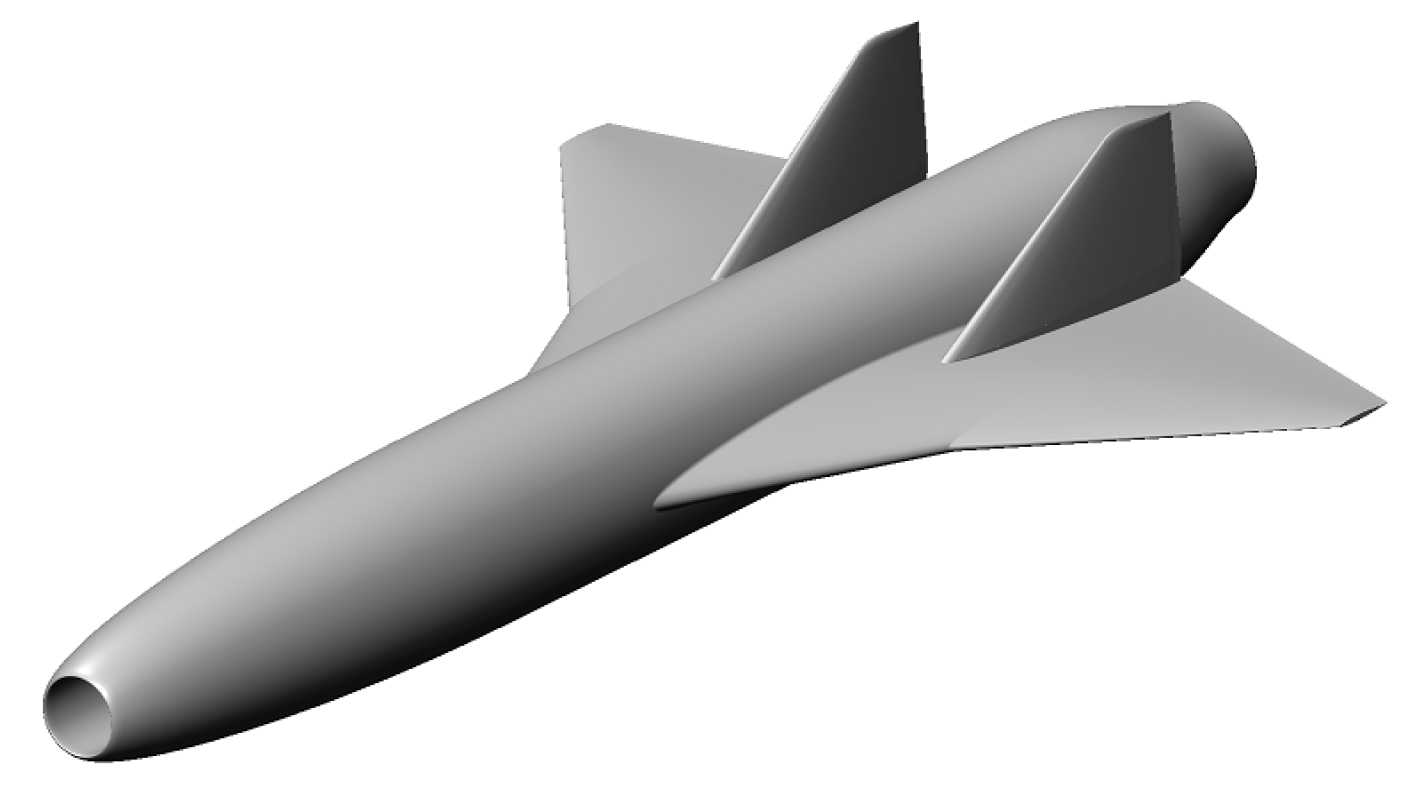
\includegraphics[width=0.95\linewidth]{Photos/Aircraft/MUFASA_Gair}
		\caption{MUFASA A.3, adapted from \citeauthor{ShaunThesis} \cite{ShaunThesis}.}
	\end{subfigure}
	\begin{subfigure}{0.48\textwidth}
		\centering
		\captionsetup{width=0.95\linewidth}
		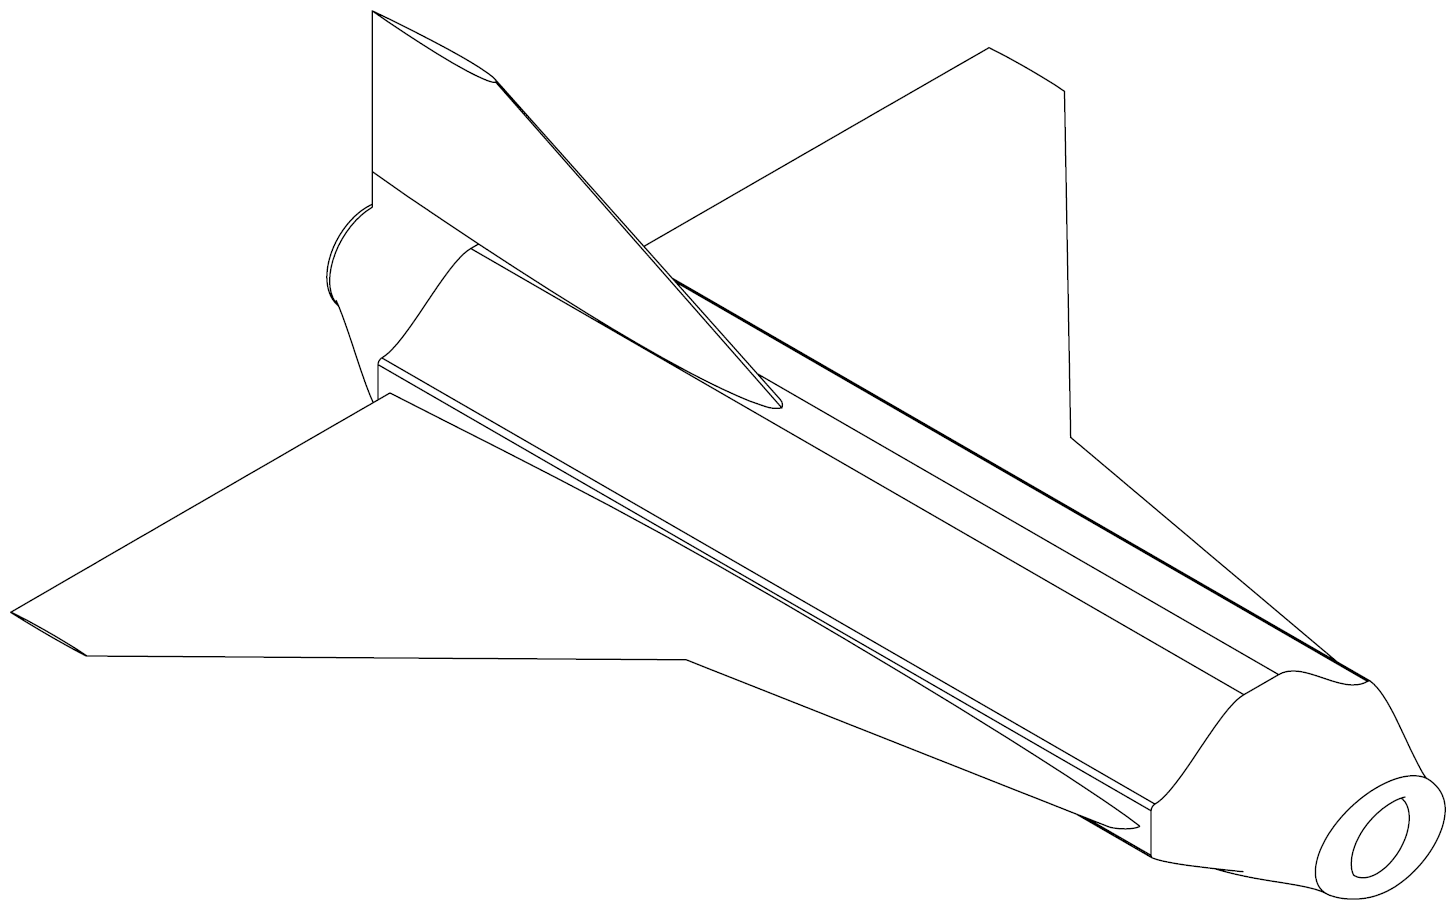
\includegraphics[width=0.95\linewidth]{Photos/Aircraft/MUFASA_ISO}
		\caption{MUFASA B.1.}
	\end{subfigure}
	\caption{MUFASA project aircraft versions (not to scale). \label{fig:aircraftComparison}}
\end{figure}

Matching the formatting of plotted results to the \LaTeX\ document they will be presented in is critically important. 
All rules provided in \Cref{sec:documentSetupFigureTableRules}, and exemplified in \cref{fig:dataExample} should be followed. 
An example of MATLAB code used to auto-format plotted data for \LaTeX\ is presented in \Cref{sec:appendixMatlabFigureCode}. 
It is also worth noting that plotted data could be directly drawn in \LaTeX\, using \LaTeX\ code, however this workflow requires first generating the plotted data in \href{https://www.python.org/}{Python} according to A. Garcia (personal communication, December 05, 2023).

\subsection{Table Creation}
Useful \LaTeX\ commands to generate tables meeting the requirements outlined in \Cref{sec:documentSetupFigureTableRules} are presented in this section. 
A useful package to generate tables with correct caption widths is \textit{threeparttable}. 
To generate correct thickness horizontal lines, the commands \verb*|\toprule|, \verb*|\midrule|, and \verb*|\bottomrule| are used. 
Manually typing table formatting is complex, and it is instead recommended to use a formatting tool, such as the \href{https://www.tablesgenerator.com/}{TablesGenerator website}. 
As an example, the code used to generate \Cref{tab:tenseBasedOnSection} is presented in \Cref{sec:appendixTables}. 


\subsection{Equations}
When coding an equation, carefully consider what is a variable and what is a label. 
Variables should be in math text, while labels should be in regular text. 
For example, in \cref{eqn:netForce}, $F_{\text{net}}$ is net force, not force as a function of variables $n \times e \times t$. 
Regular text can be inserted into an equation via the \verb*|\text{}| command. 


Sometimes equations are exceptionally long, or a matrix is too tall. Some commands that aid with unwieldy equations include \textit{smallmatrix}, \textit{sideways}, \textit{align}, and \textit{split}.	
An example of how to split a long equation is presented in \Cref{sec:appendixLongEquation}.


\LaTeX\ allows for the creation of multiple unique mathematical symbols. A comprehensive overview of possible \LaTeX\ symbols, and their associated commands, is presented in \Cref{sec:appendixLaTeXSymbols}. 

\subsection{Custom Variable Creation}
\newcommand{\ap}{ArduPilot}
Local \LaTeX\ document variables are a way to aid in typing repetitive words or numerical values. 
These custom variables also aid in document consistency when referring to repeated words or values. 
An example of using locally defined document variables is creating a command to represent the word \textit{ArduPilot}. 
Due to the letters in \textit{ArduPilot}, it is an awkward word to type and a coding shorthand is created using the command: \verb*|\newcommand{\ap}{ArduPilot}|. 
Now, by typing \verb*|\ap\|, the word \ap\ is seamlessly inserted into the text. 
Note that the \verb*|\| following the \verb*|\ap| indicates a space should be left following the word \ap.

\LaTeX\ variables also work when inserted into InkScape generated figures, as outlined in the following YouTube video: \url{https://youtu.be/r0G44lxhTwc?si=SVSKCUj6mTy4rGCN}. 
Using variables in a diagram increases writing efficiency as it reduces the need to manually regenerate diagrams to change a variable when using the workflow presented in \Cref{sec:figureCreation}. 

